\section{Μέθοδοι και Χρονοδιάγραμμα Υλοποίησης}
\begin{frame}
	\frametitle{Μέθοδοι και Χρονοδιάγραμμα Υλοποίησης}

	\centering
	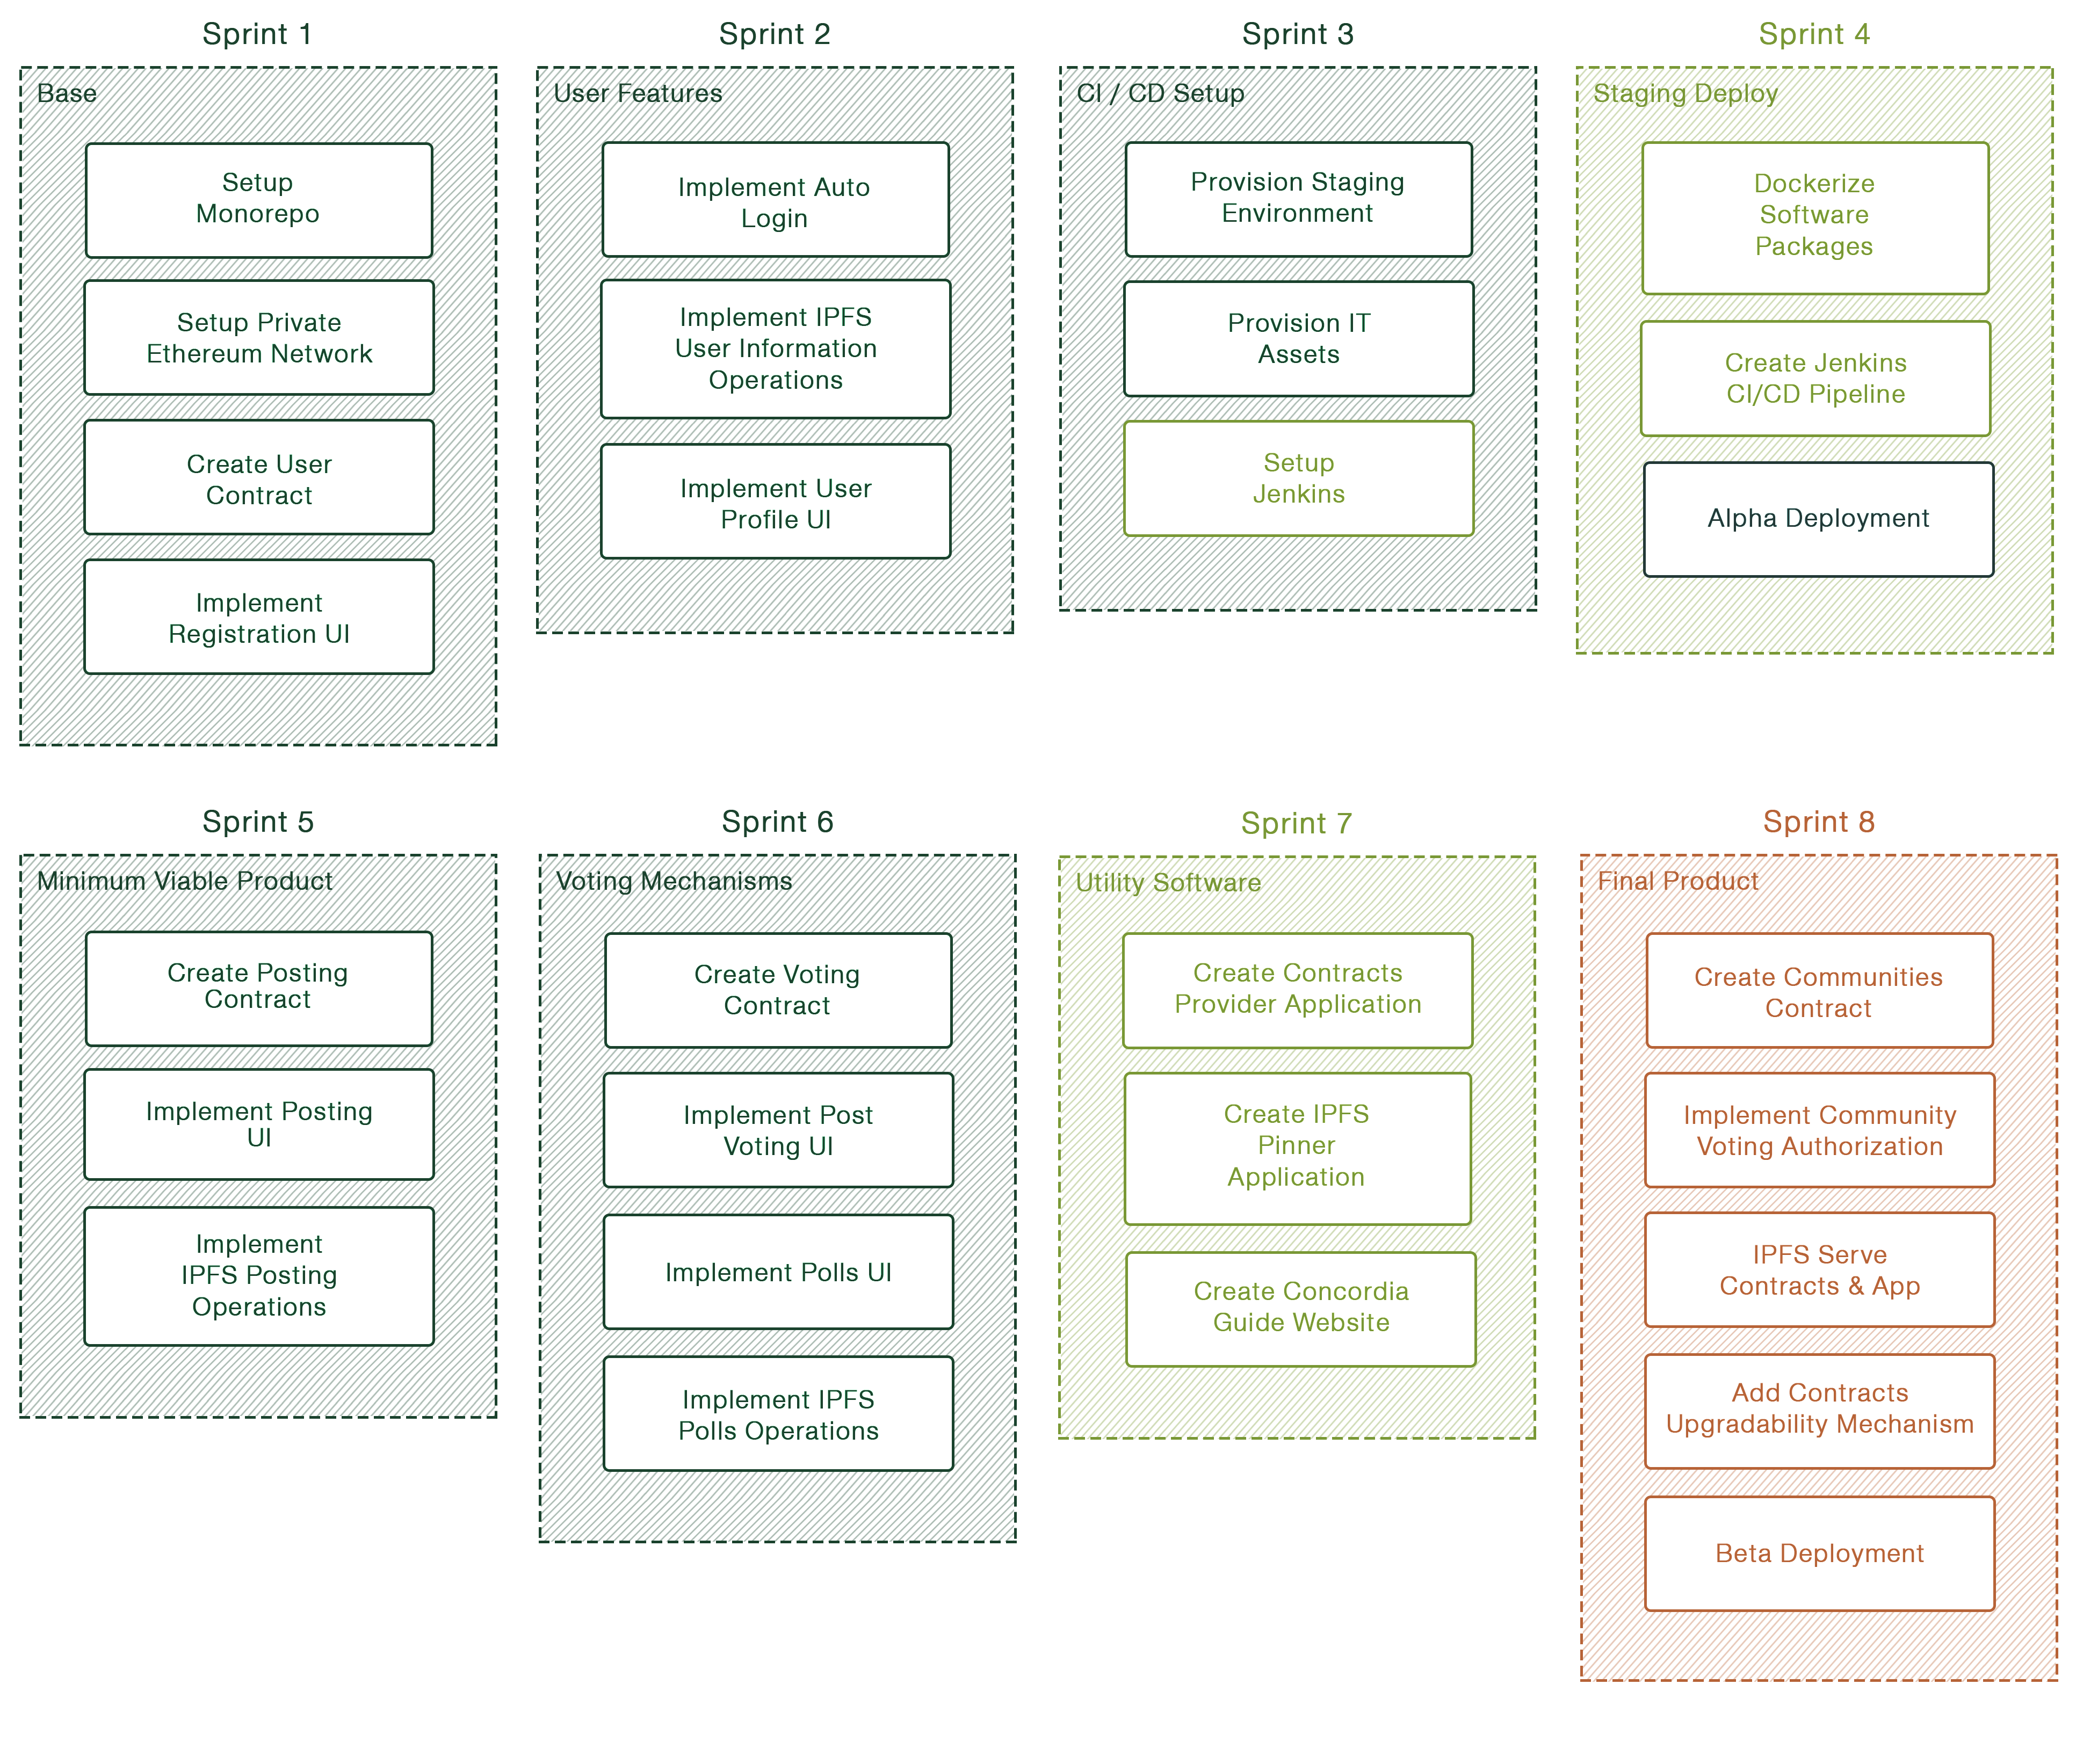
\includegraphics[width=.82\textwidth]{assets/figures/implementation-sprints.png}
\end{frame}

\note{
	Σε αυτό το μέρος της παρουσίασης θα αναλύσουμε τις μεθόδους που χρησιμοποιήθηκαν κατά την ανάπτυξη της εφαρμογής και τον χρονοπρογραμματισμό που έγινε.

	Τόσο η σχεδίαση όσο και η ανάπτυξη της εφαρμογής ακολούθησαν τις σύγχρονες μεθόδους Agile development.

	Το συνολικό έργο χωρίστηκε σε tasks. Τα tasks είναι αυτόνομα μέρη υλοποίησης που λύνουν ένα μικρό υπο-πρόβλημα της συνολικής σχεδίασης. Δημιουργήθηκαν οχτώ ομάδες, Sprints, οι οποίες αναφέρονται σε διακριτούς στόχους της πλατφόρμας και ομαδοποιούν τα tasks τα οποία συνεισφέρουν στον στόχο αυτό. Τα tasks κάθε ομάδας υλοποιήθηκαν παράλληλα. Ενώ οι ομάδες υλοποιήθηκαν διαδοχικά σε προδιαγεγραμμένο χρονικό ορίζοντα περάτωσης, καταλαμβάνοντας ένα μήνα ανάπτυξης η κάθε μία.

	Η πλειοψηφία των task αφορά στην υλοποίηση επιμέρους χαρακτηριστικών της πλατφόρμας όπως η εγγραφή ή η δημοσίευση μηνυμάτων.

	Έγινε επίσης δουλειά σε άλλα μέρη της ανάπτυξης όπως το DevOps. Για τις ανάγκες της υλοποίησης, έγινε χρήση του συστήματος CI-CD Jenkins. Το Jenkins είναι ένα αυτοματοποιημένο σύστημα ενσωμάτωσης, ελέγχου και ολοκλήρωσης λογισμικού. Με τη χρήση του CI-CD αυτοματοποιήθηκαν: το χτίσιμο (build) των εφαρμογών μας, ο έλεγχος (testing), η ενσωμάτωση που εδώ αφορά την δημοσίευση του πακεταρισμένου λογισμικού, καθώς και η εγκατάσταση (deployment).

	Λόγω χρονικών περιορισμών, αποφασίσαμε να μην προχωρήσουμε στην υλοποίηση του τελευταίου Sprint.
}
